\chapter{Аналитический раздел}
\label{cha:analysis}

\section{Постановка задачи}
Необходимо разработать программный комплекс, который позволяет автоматически определить и удалить подпись в электронном письме, содержащем текст на русском языке. Программа должна принимать на входе полный текст электронного письма и по возможности имя отправителя. В результате работы программы в тексте письма должна быть найдены строки, относящиеся к подписи. 
\section{Цель и решаемые задачи}
Целью работы является разработка метода автоматизированного удаления подписей из текстов русскоязычных электронных писем, а также его программная реализация.

Для достижения поставленной цели необходимо решить следующие задачи:
\begin{itemize}
	\item анализ предметной области;
	\item анализ существующих подходов и методов решения задач, связанных с обработкой текста на естественном языке;
	\item разработка собственного метода на основании проанализированных;
	\item разработка программного комплекса, реализующего выбранный метод;
	\item анализ эффективности работы программного продукта.
\end{itemize}
\newpage
\section{Анализ предметной области}

\subsection{Электронное письмо}

Так как объектом исследования данной работы является электронное письмо, и разрабатываемое программное обеспечение должно обрабатывать текст электронного письма, целесообразным будет рассмотреть структуру электронного письма, формат его представления,  а также требования, предъявляемые к его оформлению. Данный анализ поможет конкретизировать постановку требований к разрабатываемому методу и программному обеспечению, а также поможет установить ограничения, в рамках которых будет реализован метод.

\textbf{Структура электронного письма}

Общепринятым и повсеместно используемым протоколом обмена электронной почтой является SMTP(англ.Simple mail transfer protocol — простой протокол передачи почты). Исходя из этого, следует рассмотреть структуру электронного письма, передаваемого по протоколу SMTP.

Согласно стандарту RFC 5322 \cite{rfc5322}, который описывает формат сообщений, передаваемых путем использования электронной почты, электронное письмо, передаваемое по протоколу SMTP, состоит из следующих частей:
 

\begin{itemize}
	\item данные SMTP-конверта;
	\item заголовки письма;
	\item тело письма. 
\end{itemize}

\textbf{SMTP конверт} отправляется как серии протокольных объектов. Включает в себя адрес отправителя (куда должна быть отправлена ошибка в случае неблагоприятного события); одного или более адресов получателей; дополнительный материал, расширяющий протокол \cite{BMSTU-WIKI-SMTP}.
В большинстве случаев данная информация недоступна конечному получателю. Для возможности контролировать работоспособность системы эта информация обычно сохраняется в журналах почтовых серверов.
 
\textbf{Заголовки письма} описываются стандартом RFC 2076 — Common Internet Message Headers (общепринятые стандарты заголовков сообщений) \cite{rfc2076}.
Заголовки используются для журналирования прохождения письма и служебных пометок.В заголовка как правило содержится служебная информация о почтовых серверах, через которые прошло письмо, информация о проверке антивирусом и о том, похоже ли данное письмо на спам, а также другая служебная информация.  Поскольку заголовки являются служебной информацией, то чаще всего почтовые клиенты скрывают их от пользователя при обычном чтении писем, но также предоставляют возможность увидеть эти заголовки, если возникает потребность в более детальном анализе письма. Также заголовки письма хранят и показываемую пользователю информацию, обычно это отправитель письма, получатель, тема и дата отправки. 

\textbf{Тело письма} отделяется от заголовков пустой строкой и содержит в себе непосредственно сообщение письма.  Первоначально в спецификации SMTP было определено использование только 7-битовых символов ASCII. Но с появлением стандарта многоцелевых почтовых расширений Internet (Multipurpose Internet Mail Extensions — MIME) и превращением Internet во всемирную сеть было предложено включить в дополнительные спецификации другие наборы символов. Благодаря этому в настоящее время электронное письмо может быть отправлено практически на любом национальном языке, а к письму могут прилагаться в закодированном виде данные почти любого типа, даже такие как изображения или исполняемые файлы \cite{BMSTU-WIKI-SMTP}.

В связи с этим, в настоящее время тело многих электронных писем представляется отправителем не в виде текста с сообщением(рисунок \ref{anal:a1}), а в виде текста на языке HTML, содержащем в себе текст самого сообщения(рисунок \ref{anal:a2}). 
 
 \newpage
 
\begin{figure}[h!]
	\centering
	
\includegraphics[scale=0.4]{inc/img/a1.png}
	\caption{Электронное письмо, содержащее тело в виде текста с сообщением}
	\label{anal:a1}
\end{figure}


\begin{figure}[h!]
	\centering
	
\includegraphics[scale=0.4]{inc/img/a2.png}
	\caption{Электронное письмо, содержащее тело в виде  текста на языке HTML}
	\label{anal:a2}
\end{figure}

%Следует заметить, что 
%Сказать, что используется не только текст, поэтому %ссылки на еще один RFC

\subsection{Подпись в электронных письмах}

Подпись представляет собой набор последовательных строк в конце текста электронного письма, который добавляется автоматически с помощью почтового клиента или дописывается автором(рисунок \ref{anal:sig-example}).

\begin{figure}[h!]
	\centering
	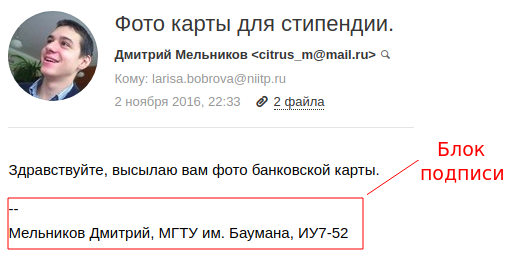
\includegraphics[width=\textwidth]{inc/img/sig-example.png}
	\caption{Пример оформления подписи в электронном письме}
	\label{anal:sig-example}
\end{figure}

Как правило, подпись содержит информацию об отправителе, например, имя отправителя, его должность, контактные данные и др. 

Подпись в электронном письме является неотъемлемым атрибутом переписки, так как наличие подписи, при условии ее правильного оформления, производит благоприятное впечатление на партнеров по общению. 
В зависимости от характера письма(личная или деловая переписка, рекламная рассылка) можно выделить ряд основных функций, которые возлагаются на подпись:

\begin{itemize}
	\item установление доверительных отношений с партнером по общению;
	\item доведение информации;
	\item ненавязчивая реклама;
	\item экономия временных затрат при автоматизации процедуры визирования сообщений. 
\end{itemize}

%Несмотря на разные форматы и правила оформления подписи, %можно выделить ряд признаков, с помощью которых будет %возможно охарактеризовать.

%Классификация из статьи


\subsection{Выводы}
На основе анализа структуры письма можно сделать вывод о том, что для текущей работы интерес будет представлять именно тело письма, а также, возможно, и некоторые заголовки.

Также следует заметить, что не существует единого стандарта для оформления подписи или ее обозначения почтовым клиентом. Как правило, оформление подписи в электронном письме может регламентироваться локальными правилами, например кодексом компании, или устоявшимися в обществе нормами. Однако, несмотря на это, подпись в электронном письме является частью текста сообщения и может иметь достаточно разные формы записи. Таким образом, можно сделать вывод о том, что задачу выделения подписи из текста электронного письма уместно будет отнести к одному из классов задач компьютерной лингвистики.

\newpage
\section{Компьютерная лингвистика: задачи и основные направления}

Компьютерная лингвистика — научное направление в области математического и компьютерного моделирования интеллектуальных процессов у человека и животных при создании систем искусственного интеллекта, которое ставит своей целью использование математических моделей для описания естественных языков \cite{wiki-comp-ling}.
Полем деятельности компьютерных лингвистов является разработка алгоритмов и прикладных программ для обработки языковой информации.

Сложность задач компьютерной лингвистики связана с тем, что естественный язык – сложная многоуровневая система
знаков, возникшая для обмена информацией между людьми, выработанная в процессе практической деятельности человека, и постоянно изменяющаяся в связи с этой деятельностью. Другая сложность разработки методов компьютерной лингвистики связана с многообразием естественных языков, существенными отличиями их лексики, морфологии, синтаксиса, разные языки предоставляют разные способы выражения одного и того же смысла \cite{Posobie}.

Область приложений компьютерной лингвистики постоянно расширяется, однако можно выделить наиболее известные прикладные задачи, решаемые с помощью ее инструментов\cite{Posobie}:
\begin{itemize}
	\item машинный перевод;
	\item реферирование текста;
	\item аннотирование текста;
	\item классификация текстов;
	\item кластеризация текстов;
	\item формирование ответов на вопросы;
	\item автоматизация подготовки и редактирования текстов на естественном языке;
	\item автоматическая генерация текстов на естественном языке;
	\item извлечение информации из текстов;
	\item распознавание и синтез звучащей речи.
\end{itemize}

\textbf{Машинный перевод} \cite{machine-translation} является самым ранним приложением компьютерной лингвистики, вместе с которым развивалась и сама эта область. Первые программы, использующие машинный перевод, были построены более 50 лет назад и были основаны на простейшей стратегии пословного перевода. Однако сейчас, данное направление достаточно хорошо развито: программы машинного перевода используются повсеместно с применение самых последних технологий и методов.

\textbf{Реферирование текста} – сокращение его объема и получение его краткого изложения – реферата (свернутого содержания), что делает более быстрым поиск в коллекциях документов. Общий реферат может составляться также для нескольких близких по теме документов. Основным методом автоматического реферирования до сих пор является отбор наиболее значимых предложений реферируемого текста, для чего обычно сначала вычисляются ключевые слова текста и рассчитывается коэффициент значимости предложений текста.

Близкая к реферированию задача – \textbf{аннотирование текста} документа, т.е.составление его аннотации. В простейшей форме аннотация представляет собой перечень основных тем текста, для выделения которых могут использоваться процедуры индексирования.

При создании больших коллекций документов актуальны задачи
\textbf{классификации} и \textbf{кластеризации} текстов с целью создания классов близких по теме документов \cite{vasiliev-krivenko}. Классификация означает отнесение каждого документа к определенному классу с заранее известными параметрами, а кластеризация – разбиение множества документов на кластеры, т.е. подмножества тематически близких документов. Для решения этих задач применяются методы машинного обучения, в связи с чем эти прикладные задачи называют Text Mining и относят к научному направлению, известному как Data Mining, или интеллектуальный анализ данных \cite{data-mining}.

Еще одна относительно новая задача, связанная с информационным поиском – \textbf{формирование ответов на вопросы} (Question Answering) \cite{qa}. Эта задача решается путем определения типа вопроса, поиском текстов, потенциально содержащих ответ на этот вопрос, и извлечением ответа из этих текстов.

Совершенно иное прикладное направление, которое развивается хотя и медленно, но устойчиво – это \textbf{автоматизация подготовки и редактирования
текстов на ЕЯ}. Одним из первых приложений в этом направлении были программы автоматической определения переносов слов и программы орфографической проверки текста (спеллеры, или автокорректоры). Несмотря на кажущуюся простоту задачи переносов, ее корректное решение для многих языков (например, английского) требует знания морфемной структуры слов соответствующего языка, а значит, соответствующего словаря.

Все более актуальная прикладная задача, часто относимая к направлению Text Mining – это \textbf{извлечение информации} из текстов, или Information Extraction \cite{information-extraction}, что требуется при решении задач экономической и производственной аналитики. Для
этого осуществляется выделение в тесте ЕЯ определенных объектов – именованных сущностей (имен, персоналий, географических названий), их отношений и связанных
с ними событий. Как правило, это реализуется на основе частичного синтаксического анализа текста, позволяющего выполнять обработку потоков новостей от информационных агентств. Поскольку задача достаточно сложна не только
теоретически, но и технологически, создание значимых систем извлечения информации из текстов осуществимо в рамках коммерческих компаний.


Как уже было сказано ранее, подпись в электронном письме содержится непосредственно в тексте письма, то есть является его частью. Полагаясь на данный факт и специфику задачи, можно сделать вывод о том, что строки текста электронного письма можно рассматривать с точки зрения принадлежности одному из двух классов: класс строк, содержащихся в подписи, и другие строки текста письма. На основании данного утверждения можно предположить, что данную задачу уместно рассматривать именно как задачу классификации множества строк текста электронного письма.
Поэтому далее следует рассмотреть существующие методы и подходы, применяемые для решения задача классификации в области обработки текстов на естественном языке. 

\newpage
\section{Анализ существующих подходов и методов классификации текстов на естественном языке}

Для решения задач классификации, в том числе и в области обработки текстов на естественном языке, наиболее успешно применяются методы, использующие нейронные сети \cite{golovko-neural-networks}. Их использование для решения задачи классификации состоит в указании принадлежности входного образа, представленного вектором входных признаков, одному или нескольким заранее определенным классам.

Построение эффективной нейросетевой модели, решающей задачи классификации, можно разделить на следующие основные этапы \cite{golovko-neural-networks}:
\begin{itemize}
	\item получение исходных данных из множества объектов, подлежащих классификации;
	\item предварительная обработка исходных данных и формирование обучающей выборки для обучения нейронной сети;
	\item разработка структуры нейронной сети: задание входов, выходов, числа слоев сети и нейронов в каждом слое;
	\item обучение нейронной сети для построения модели классификатора;
	\item тестирование и оценка качества работы нейросетевой модели.
\end{itemize}

При неудовлетворительных результатах оценки модели необходимо вернуться к одному из этапов и выполнить все последующие этапы в указанной последовательности.

Процесс получение исходных данных, которые необходимо использовать для обучения, определяется прежде всего спецификой задачи, а также требованиями к разрабатываемому программному обеспечению. Однако, для обучения классификатора недостаточно просто полученных исходных данных, так как модель классификатора, использующего методы машинного обучения, должна принимать на вход вектор числовых значений, который описывает точку в пространстве признаков. Используя множество таких векторов, можно обучить модель разделять все пространство признаков на определенное количество областей. В связи с этим возникает необходимость предварительной обработки исходных данных с целью приведения их к форме, пригодной для передачи на вход классификатора. 

\subsection{Предварительная обработка данных}
 В зависимости о типа задачи и исходного формата входных данных можно выделить основные подходы, применяемые для предварительной обработки данных и приведения их к необходимому виду:
 
 \begin{itemize}
 	\item использование словарей и частотного анализатора;
 	\item использование векторного представления слов;
 	\item выделения множества признаков, описывающих классифицируемые объекты;
 \end{itemize}

Суть подхода с использованием \textbf{словарей и частотного анализатора} заключается в том, что перед обучением классификатора из множества учебных текстов определенным образом выделяются слова, т.е. формируется словарь. Затем на основании данного словаря с использованием частотного анализатора для текста строится вектор, который описывает частотные характеристики для всех слов, содержащихся в тексте. Схема частотного анализатора представлена на рисунке \ref{anal:freq-anal}).

\begin{figure}[h!]
	\centering
	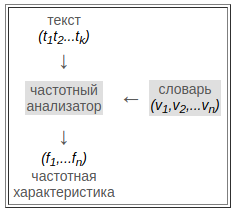
\includegraphics[scale=0.8]{inc/img/freq-analis.png}
	\caption{Схема частотного анализатора}
	\label{anal:freq-anal}
\end{figure}

Частотный анализатор определяет для каждого слова $v_i$ из словаря $V$ его частоту вхождения $f_i$ в данный текст $t$. Частотная характеристика это вектор $f=(f_1,...,f_n)\in F$, длина которого равна количеству слов в словаре $V$, каждая компонента $f_i$ это целое неотрицательное число:

\begin{equation}
f_i = \sum_{j=0}^{k} e(v_i, t_j); e(v_i, t_j)= \left\{ \begin{array}{ll}
0, & v_i \neq t_j\\
1, & v_i=t_j
\end{array} \right.
\end{equation}
\vspace{\baselineskip}

Другими словами - для каждого слова $v_i \in V$	определяется число его вхождений $f_i \geq 0$ в данный текст $t=t_1t_2t_3...t_k$. Частотную характеристику $f$ можно рассматривать как точку в пространстве признаков  $F$, соответствующую тексту  $t$. Таким образом, на вход частотного анализатора подается текст $t$ и словарь $V$, на выход выдается точка в пространстве признаков $F$.

Словарь - важная часть модели классификатора, поэтому он должен удовлетворять следующим требованиям \cite{borisov}:
 \begin{itemize}
	\item Словарь должен состоять из слов, имеющих четко определенное значение, чтобы результат частотного анализа содержал минимум шума;
	\item Словарь должен содержать достаточно слов, чтобы частотный анализ был информативен;
	\item Словарь должен быть небольшим, чтобы процедура частотного анализа могла быть выполнена за приемлемое время;
\end{itemize}

Составить словарь, удовлетворяющий этим требования, можно используя известные лингвистические закономерности. В качестве примера для такой закономерности можно привести закон Бредфорда \cite{lande}.


\vspace{\baselineskip}
Подход, использующий \textbf{векторные представления слов}, заключается в следующем: процесс предварительной обработки данных начинается с обучения нейронной сети, которая принимает на вход большой корпус текстовых данных и сопоставляет каждому слову вектор, выдавая координаты слов на выходе. Векторное представление основывается на контекстной близости: слова, встречающиеся в тексте рядом с одинаковыми словами, в векторном представлении будут иметь близкие координаты векторов-слов \cite{word2vec}. Минусом данного подхода является то, что после получения векторного представления слов возникает задача объединения всех представлений, входящих в классифицируемые объекты(тексты, предложения), в единый вектор, пригодный для передачи на вход классификатора.
\vspace{\baselineskip}

Также решить проблему предварительной обработки данных можно не прибегая к использованию словарей или больших корпусов текстовых данных. Для этого можно воспользоваться походом, который заключается в \textbf{выделении множества признаков}, которые будут пригодны для классификации объектов в рамках решаемой задачи.

В качестве примера можно рассмотреть применение данного подхода в статье А.С.Катасёва, Д.В.Катасёвой, А.П.Кирпчникова \cite{spam-filter}, в которой авторами описывается метод реализации спам-фильтра электронных сообщений на основе нейросетевого классификатора. Для классификации сообщений, в своей работе авторы статьи провели предварительную обработку исходных данных(текстов писем), представив их в качестве векторов признаков. Для этого они выделили следующие признаки, которые, по их мнению, влияют на результат классификации писем на категории "спам"/"не спам":
\begin{itemize}
	\item частота встречаемости слов верхнего регистра;
	\item частота встречаемости цифр в письме;
	\item количество разных цветов в тексте письма;
	\item размер текста письма;
	\item количество пустых строк в тексте письма;
\end{itemize}

\vspace{\baselineskip}

%http://neuronus.com/theory/931-sposoby-normalizatsii-peremennykh.html
Стоит также заметить, что предварительная обработка данных включает в себя помимо представления исходных данных в формате числового вектора еще и \textbf{нормализацию} значений полученного вектора. Под нормализацией понимается такое преобразование вектора значений, в результате которого все значения вектора принимают значений в диапазоне от 0 до 1. Нормализация данных позволяет привести все используемые числовые значения переменных к одинаковой области их изменения, благодаря чему появляется возможность свести их вместе в одной нейросетевой модели \cite{AI-portal}.
Чтобы выполнить нормализацию данных, нужно точно знать пределы изменения значений соответствующих переменных. Тогда им и будут соответствовать границы интервала нормализации. Когда точно установить пределы изменения переменных невозможно, они задаются с учетом минимальных и максимальных значений в имеющейся выборке данных.
Методы нормализации принято разделять на две следующие группы \cite{AI-portal}:
\begin{itemize}
	\item линейная нормализация;
	\item нелинейная нормализация.
\end{itemize}


\subsection{Алгоритмы классификации}
Алгоритмы классификации можно разделить на две группы:
\begin{itemize}
	\item алгоритмы классификация с учителем;
	\item алгоритмы классификации без учителя. 
\end{itemize}

Алгоритмы \textbf{классификации с учителем} сортируют объекты классифицируемого множества по заранее известным категориям(классам). В роли учителя выступает выборка объектов, для которых заранее известна принадлежность той или иной категории, называемая обучающим множеством \cite{Posobie}. 
Алгоритмы классификации называют по имени метода обучения, положенного в его основу. К наиболее известным алгоритмам классификации с учителем относятся следующие \cite{Posobie}:
\begin{itemize}
	\item Алгоритм "наивной" байесовской классификации;
	\item Алгоритм k-ближайших соседей;
	\item Алгоритм опорных векторов.
	%\item Алгоритм Роккио;
	%\item Алгоритм деревьев принятия решений. 
\end{itemize}

Алгоритмы \textbf{классификации с учителем} анализируют
коллекцию объектов с целью разбиения их на группы так, чтобы внутри одной группы оказывались объекты наиболее родственные в некотором смысле, а различные - попадали в различные группы. При этом отсутствует «учитель» - обучающее подмножество документов и заранее известное множество категорий (классов). В общем случае алгоритм классификации без учителя - алгоритм кластеризации - должен самостоятельно принимать решения о количестве и составе кластеров, то есть групп родственных объектов \cite{Posobie}.

Так как в данной работе четко определены классы, согласно которым следует классифицировать строки электронного письма, то следует более детально рассмотреть алгоритмы классификации с учителем и не останавливаться на подробном разборе алгоритмов классификации без учителя, так как задача кластеризации в данной работе не стоит.

\vspace{\baselineskip}
\textbf{Алгоритм "наивной" байесовской классификации}
Алгоритм "наивной" байесовской классификации(НБА) - это алгоритм классификации, основанный на теорема Байеса \cite{Bayes} c допущением о независимости признаков. То есть алгоритм НБА не предполагает, что наличие какого-либо признака в классе не зависит от наличия какого-либо другого признака. Даже если какие-то признаки и зависят друг от друга, то считается, что они вносят независимый вклад в вероятность принадлежности классифицируемого объекта определенному классу. В связи с данным допущением алгоритм и называется "наивным". 

Рассмотрим объект $O$. А также множество классов $C$, к одному из которых следует отнести объект $O$. Необходимо найти такой класс $c$ из множества $C$, при котором вероятность для данного объекта была бы максимальна. Математически это можно записать в следующем виде:

\begin{equation}
c = arg\max_{C} P(C|O).
\end{equation}

\vspace{\baselineskip}
Для вычисления  P($C$|$O$) можно воспользоваться теоремой Байеса и перейти к косвенным вероятностям:

\begin{equation}
P(C|O) = \frac{P(O|C)P(C)}{P(O)}
\end{equation}

\vspace{\baselineskip}
Так как в задачах классификации объект $O$ представляется вектором признаков ($o_1$$o_1$...$o_n$), то предыдущая формула примет вид:

\begin{equation}
P(C|o_1o_2...o_n) = \frac{P(o_1o_2...o_n|C)P(C)}{P(o_1o_2...o_n)}
\end{equation}

\vspace{\baselineskip}
C учетом "наивного" допущения о том, что переменные $o_i$ зависят только от класса $С$ и не зависят друг от друга, можно переписать числитель в следующем виде:

\begin{equation}
P(o_1o_2...o_n|C)P(C) = P(C)\prod\limits_{i}P(o_i|C)
\end{equation}

\vspace{\baselineskip}
В итоге (1.2) примет вид:

\begin{equation}
c = arg\max_{c \in C} P(c|o_1o_2...o_n) = arg\max_{c \in C} P(c)\prod\limits_{i}P(o_i|C)
\end{equation}

Соответственно, под тренировкой классификатора понимается вычисление значений P($c$) и P($o_i$|$c$).

К плюсам данного алгоритма можно отнести возможность его применения для решения задач многоклассовой классификации, высокую скорость обучения классификатора, а также тот факт, что при выполнении допущения о независимости алгоритм НБА может превосходить другие алгоритмы, при этом требуя меньший объем обучающей выборки. Однако, если в тестовом наборе присутствует некоторое значение категорийного признака, которое не встречалось в обучающей выборке, тогда модель присвоит нулевую вероятность этому значению, что негативно скажется на результатах прогноза. Также стоит заметить, что в реальности наборы полностью независимых признаков встречаются крайне редко, поэтому допущение о независимости признаков будет выполняться редко при решении реальных задач.

\vspace{\baselineskip}
\textbf{Алгоритм $k$-ближайших соседей}
Алгоритм $k$-ближайших соседей использует гипотезу компактности векторного пространства, которая заключается в том, что объекты одного класса образуют в пространстве признаков компактную область, причем области разных классов не пересекаются. Тогда можно ожидать, что тестовый объект будет иметь такую же метку класса, как и окружающие его объекты из обучающего множества. Данный алгоритм относит объект к преобладающему классу среди k его соседей. При $k$=1 алгоритм относит объект к классу самого ближайшего ему объекта.

Суть работы алгоритма можно рассмотреть на примере, представленном на рисунке \ref{anal:k-neigbors}.

\begin{figure}[h!]
	\centering
	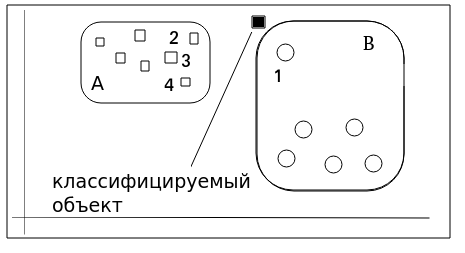
\includegraphics[width=\textwidth]{inc/img/k-neignbors.png}
	\caption{Геометрическая интерпретация алгоритма $k$-ближайших соседей}
	\label{anal:k-neigbors}
\end{figure}

Пусть имеется множество объектов, принадлежащих двум классам: A и B. При $k$ = 1, классифицируемый объект будет отнесен к классу B, так как ближе всего классифицируемый объект располагается к объекту 1, принадлежащему классу B.
Однако, при $k$=4, классифицируемый объект будет отнесен к классу А, так как среди четырех объектов, минимально удаленных от классифицируемого объекта, три объекта будут принадлежать классу А(объекты 2,3,4).

Перед тем, как определять $k$ наименее удаленных объектов, необходимо определить функцию дистанции. Классическим вариантом функции дистанции является дистанция в евклидовом пространстве \cite{distance}:

\begin{equation}
d(p,q) = \sqrt{\sum_{k=1}^{n}(p_k-q_k)^2},
\end{equation}

где $p=(p_1,...,p_n)$ и $q=(q_1,...,q_n)$ - точки в евклидовом пространстве размерности $n$.

При использовании данного алгоритма основной задачей, которую необходимо решить, является выбор значения $k$.
Если выбрать значение $k$ слишком малым, то есть опасность, что единственным ближайшим объектом окажется «выброс», т.е. объект с неправильно определённым классом, и он даст неверное решение. Казалось бы, увеличивая
значение параметра $k$, можно понизить вероятность случайного попадания на такие «выбросы» в качестве ближайших соседей исследуемого объекта. Но здесь возникает другая опасность. Чтобы понять в чём она заключается, рассмотрим случай, когда $k$ равно общему числу объектов N. Понятно, что тогда в этом случае объект будет отнесен к классу, который имеет наибольшее количество объектов, и расстояние до исследуемого объекта не будет играть вообще никакой роли. На практике чаще всего полагают $k=\sqrt{N}$.

К плюсам данного алгоритма можно отнести то, что он подходит для решения задачи многоклассовой классификации. Однако применение данного алгоритма осложняется необходимостью подбора значения $k$, а также низкой скоростью классификации, по сравнению с НБА или алгоритмом опорных векторов.


\vspace{\baselineskip}
\textbf{Алгоритм опорных векторов}

Данный алгоритм ищет в векторном пространстве объектов разделяющую гиперплоскость между двумя классами, максимально удаленную от всех точек обучающего множества (рисунок \ref{anal:SVM}). 

\newpage
\begin{figure}[h!]
	\centering
	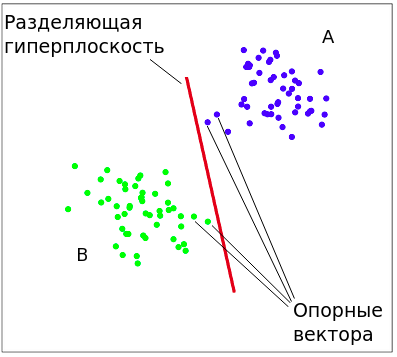
\includegraphics[scale=0.7]{inc/img/SVM.png}
	\caption{Геометрическая интерпретация алгоритма опорных векторов}
	\label{anal:SVM}
\end{figure}

Расстояние между найденной гиперплоскостью и ближайшей точкой данных называется зазором классификации. В алгоритме опорных векторов разделяющая гиперплоскость полностью определяется небольшим подмножеством объектов. Элементы данного подмножества называются опорными векторами. 



Пусть имеется обучающая выборка: ($x_1$, $y_1$),...,($x_m$,$y_m$), $x_i$ $\in \mathbf{R}^n$, $y_i \in \{-1,1\}$.
Алгоритм опорных векторов строит классифицирующую функцию:

\begin{equation}
f(\vec x) = sign(\vec w^T \vec x + b), 
\end{equation}

где 

\begin{itemize}
	\item $\vec w^T$ - вектор нормали к разделяющей поверхности;
	\item$ \vec x$ - вектор-представление классифицируемого объекта;
	\item $b$ - параметр сдвига.
\end{itemize}

Значение  функции классификатора -1 соответствует одному классу, а +1 - другому, 

Далее необходимо выбрать такие $w$ и $b$, которые максимизируют расстояние до каждого класса. Можно подсчитать, что данное расстояние равно $\frac{1}{\Vert w \Vert}$ (рисунок \ref{anal:w}).

\begin{figure}[h!]
	\centering
	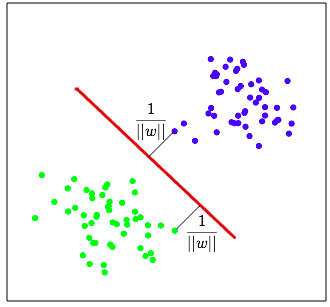
\includegraphics[scale=0.8]{inc/img/w.png}
	\caption{Расстояние от каждого класса до гиперплоскости}
	\label{anal:w}
\end{figure}

Проблема нахождения максимума $\frac{1}{\Vert w \Vert}$ эквивалентна проблеме нахождения минимума ${\Vert w \Vert}^2$.
Данное условие можно записать в виде задачи оптимизации:

\begin{equation}
\left\{ \begin{array}{ll}
 arg\min_{w,b} {\Vert w \Vert}^2,\\
y_i(\vec w^T \vec x + b) \geq 1, i = 1,...,m.
\end{array} \right.
\end{equation}

\vspace{\baselineskip}
которая является стандартной задачей квадратичного программирования и решается с помощью множителей Лагранжа \cite{Lagrange}.

На практике редко встречаются случаи, когда исследуемое множество линейно разделимо. Пример линейной неразделимости показан на рисунке \ref{anal:non-linear}.

\begin{figure}[h!]
	\centering
	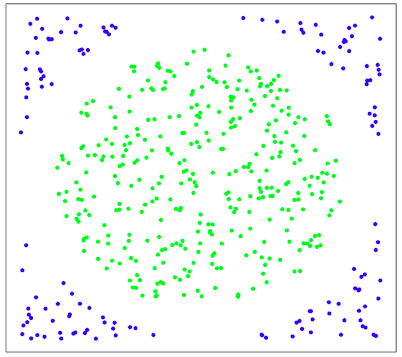
\includegraphics[scale=0.7]{inc/img/non-linear.png}
	\caption{Линейно неразделимое множество}
	\label{anal:non-linear}
\end{figure}

В этом случае поступают следующим образом: все элементы обучающей выборки вкладываются в пространство $X$ более высокой размерности с помощью специального отображения: $\varphi: \mathbf{R}^n \to X$. При этом отображение $\varphi$ выбирается таким образом, чтобы в новом пространстве $X$ выборка была линейно разделима.

В таком случае классифицирующая функция примет следующий вид:

\begin{equation}
f(\vec x) = sign(\vec w^T \varphi(\vec x) + b)
\end{equation}

Выражение $k(x, x') = (\varphi(x),\varphi(x'))$ называется ядром классификатора. С математической точки зрения ядром может служить любая положительно определенная симметричная функция двух переменных \cite{Vorontsov-lections}.
Выбор ядра влияет на точность работы классификатора.

К плюсам данного метода можно отнести хорошие показатели работы алгоритма в случаях линейной разделимости. Однако, при не выполнении условия линейной разделимости, необходимо прибегать к подбору параметров ядра для получения наилучших результатов, что требует большое количество времени, так как при каждом новом подборе параметра выполняется переобучение классификатора. Также следует обратить внимание, что в классическом варианте данный алгоритм подходит только для решения задач бинарной классификации.

%\vspace{\baselineskip}
%\textbf{Алгоритм деревьев принятия решений}

\subsection{Параметры для оценки качества работы классификатора}

В простейшем случае метрикой для оценки качества работы классификатора может быть доля объектов, по которым классификатор принял правильное решение:

\begin{equation}
Accuracy = \frac{P}{N},  
\end{equation}

\vspace{\baselineskip}
где $P$ - количество объектов, по которым классификатор принял правильное решение, $N$ - размер тестовой выборки.

Тем не менее, данная метрика имеет одну особенность, которую необходимо учитывать. Она присваивает всем объектам одинаковый вес, что может быть не корректно в случае, если распределение объектов в обучающей выборке сильно смещено в сторону какого-то одного или нескольких классов. В этом случае у классификатора есть больше информации по этим классам и соответственно в рамках этих классов он будет принимать более адекватные решения. Для решения данной проблемы можно воспользоваться специально подобранной сбалансированной обучающей выборкой, однако рекомендуется для оценки качества работы классификатора использовать другие метрики.

Одними из таких метрик являются \textbf{точность}(precision) и \textbf{полнота}(recall).
Точность системы в пределах класса – это доля объектов, действительно принадлежащих данному классу относительно всех объектов, которые система отнесла к этому классу. Полнота системы – это доля найденных классификатором объектов, принадлежащих классу относительно всех объектов этого класса в тестовой выборке. Для расчета значения данных параметров можно воспользоваться таблицей контингентности(рисунок \ref{anal:prec-rec-table}), которая составляется отдельно для каждого класса.

\begin{figure}[h!]
	\centering
	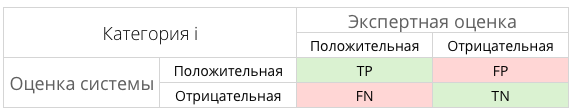
\includegraphics[width=\textwidth]{inc/img/prec-rec-table.png}
	\caption{Таблица контингентности}
	\label{anal:prec-rec-table}
\end{figure}

\newpage
В данной таблице содержится информация о том, сколько раз система приняла верное и сколько раз неверное решение при классификации объектов заданного класса. А именно:

\begin{itemize}
	\item TP - истинно-положительные;
	\item FP - ложно-положительные;
	\item TN - истинно-отрицательные;
	\item FN - ложно-отрицательные.
\end{itemize}

Тогда, точность и полнота определяются следующим образом:

\begin{equation}
Precision = \frac{TP}{TP+FP} 
\end{equation}

\begin{equation}
Recall = \frac{TP}{TP+FN}
\end{equation}

\vspace{\baselineskip}
Очевидно, что чем выше точность и полнота, тем более качественной является работа системы. Однако, максимальная точность и полнота не достижимы одновременно, поэтому приходится искать некий баланс. Для этого разумным является ввести какую-то одну метрику, которая объединяла бы в себе информацию о полноте и точности разрабатываемого классификатора. Одной из таких метрик является \textbf{F-мера}, которая представляет собой гармоническое среднее \cite{Posobie} между точностью и полнотой. Она стремится к нулю, если точность или полнота стремится к нулю. F-мера рассчитывается по следующей формуле:

\begin{equation}
F = 2\frac{Precison * Recall}{Precision+Recall}
\end{equation}

\vspace{\baselineskip}
В вычислении F-меры для задачи классификации есть два основных подхода:

\begin{itemize}
	\item Суммарный: результаты по всем классам сводятся в единую таблицу, по которой затем вычисляется F-мера;
	\item Средний: для каждого класса F-мера рассчитывается отдельно, затем на основании полученных значений вычисляется среднее арифметическое значение F-меры для всех классов.
\end{itemize}

\newpage
\section{Выводы}
В аналитическом разделе была определена цель и решаемые задачи, проведен анализ предметной области. В результате проведенного анализа был сделан вывод о том, что данная задача относится к области задач компьютерной лингвистики, а именно, к классу задач классификации. В связи с этим были также рассмотрены существующие методы и подходы, используемые для решения задач классификации.

В связи с тем, что подпись в электронном письме содержится непосредственно в его теле, то будет разумным ввести ограничение к разрабатываемому ПО, которое заключается в том, что на вход программы будет подаваться текст письма и информация из его заголовков.

Так как для работы разрабатываемого классификатора необходимо провести предварительную обработку входных данных, то в случае данной задачи наиболее подходящим будет подход, который основан на выделении множества признаков, которые будут характеризовать строки письма с точки зрения принадлежности выделенным классам ("подпись"/"не подпись"), что позволит также использовать англоязычные письма для обучения классификатора. Другие подходы, в отличие от описанного, требуют большого корпуса размеченных данных, а также большого количества именно русскоязычных писем для составления словарей. Также следует заметить, что подпись в электронных письмах часто содержит имена собственные, сокращения, а также другую информацию, например, номера телефонов, url-адреса. Данный факт также осложняет применение подхода, использующего словари.

На основании проведенного анализа существующих алгоритмов классификации, можно сделать вывод о том, что все они подходят для решения задач бинарной классификации. Однако, сложно выделить один наиболее подходящий для реализации поставленной задачи, так как качество работы данных алгоритмов классификации зависит от различных параметров, таких как размер обучающей выборки, независимость выделенных параметров, соотношение количества объектов того или иного класса в обучающей выборке. В связи с этим предлагается проверить работу всех описанных алгоритмов в рамках данной работы, а затем оценить результаты с помощью параметров, описанных в конце аналитического раздела. На основании полученных результатов можно будет сделать вывод о том, какой из алгоритмов является наиболее подходящим для решения данной задачи.
%%% Local Variables:
%%% mode: latex
%%% TeX-master: "rpz"
%%% End:
